\documentclass{article}

\usepackage{fancyhdr}
\usepackage{extramarks}
\usepackage{amsmath}
\usepackage{amsthm}
\usepackage{amsfonts}
\usepackage{amssymb}
\usepackage{xparse}
\usepackage{tikz}
\usepackage{graphicx}
\usepackage[plain]{algorithm}
\usepackage{algpseudocode}
\usepackage{listings}
\usepackage{hyperref}
\usepackage[per-mode = fraction]{siunitx}
\usepackage{calc}

\usetikzlibrary{automata,positioning}

\hypersetup{
    colorlinks=true,
    linkcolor=blue,
    filecolor=magenta,
    urlcolor=blue,
    }

\urlstyle{same}

%
% Basic Document Settings
%

\topmargin=-0.45in
\evensidemargin=0in
\oddsidemargin=0in
\textwidth=6.5in
\textheight=9.0in
\headsep=0.25in

\linespread{1.1}

\pagestyle{fancy}
\lhead{\hmwkAuthorName}
\chead{\hmwkClass\ (\hmwkClassInstructor,\ \hmwkClassTime): \hmwkTitle}
\rhead{\firstxmark}
\lfoot{\lastxmark}
\cfoot{\thepage}

\renewcommand\headrulewidth{0.4pt}
\renewcommand\footrulewidth{0.4pt}

\setlength\parindent{0pt}
\allowdisplaybreaks
%
% Title Page
%

\title{
	\vspace{2in}
	\textmd{\textbf{\hmwkClass:\ \hmwkTitle}}\\
	\normalsize\vspace{0.1in}\small{Due\ on\ \hmwkDueDate\ at \hmwkDueTime}\\
	\vspace{0.1in}\large{\textit{\hmwkClassInstructor,\ \hmwkClassTime}}
	\vspace{3in}
}
\author{\textbf{\hmwkAuthorName}}
\date{\hmwkCompletionDate}

%
% Create Problem Sections
%

\newcommand{\enterProblemHeader}[1]{
	\nobreak\extramarks{}{Problem #1 continued on next page\ldots}\nobreak{}
	\nobreak\extramarks{Problem #1 (continued)}{Problem #1 continued on next page\ldots}\nobreak{}
}

\newcommand{\exitProblemHeader}[1]{
	\nobreak\extramarks{Problem #1 (continued)}{Problem #1 continued on next page\ldots}\nobreak{}
	\nobreak\extramarks{Problem #1}{}\nobreak{}
}

%
% Homework Problem Environment
%
\NewDocumentEnvironment{hwkProblem}{m m s}{
	\section*{Problem #1: #2}
	\enterProblemHeader{#1}
	\setcounter{partCounter}{1}
}{
	\exitProblemHeader{#1}
	\IfBooleanF{#3} % if star, no new page
		{\newpage}
}

% Alias for the Solution section header
\newcommand{\hwkSol}{\vspace{\baselineskip / 2}\textbf{\Large Solution}\vspace{\baselineskip / 2}}

% Alias for the Solution Part subsection header
\newcounter{partCounter}
\newcommand{\hwkPart}{
	\vspace{\baselineskip / 2}
	\textbf{\large Part \Alph{partCounter}}
	\vspace{\baselineskip / 2}
	\stepcounter{partCounter}
}

%
% Various Helper Commands
%

% Such That
\newcommand{\st}{\text{s.t.}}

% Useful for algorithms
\newcommand{\alg}[1]{\textsc{\bfseries \footnotesize #1}}

% For derivatives
\newcommand{\deriv}[1]{\frac{\mathrm{d}}{\mathrm{d}x} (#1)}

% For partial derivatives
\newcommand{\pderiv}[2]{\frac{\partial}{\partial #1} (#2)}

% Integral dx
\newcommand{\dx}{\mathrm{d}x}
\newcommand{\dy}{\mathrm{d}y}

% Probability commands: Expectation, Variance, Covariance, Bias
\newcommand{\e}[1]{\mathrm{e}#1}
\newcommand{\E}{\mathrm{E}}
\newcommand{\Var}{\mathrm{Var}}
\newcommand{\Cov}{\mathrm{Cov}}
\newcommand{\Bias}{\mathrm{Bias}}

% Defining Units that are not in the SI base
\DeclareSIUnit\bar{bar}
\DeclareSIUnit\ft{ft}
\DeclareSIUnit\dollar{\$}
\DeclareSIUnit\cent{\text{\textcent}}
\DeclareSIUnit\c{\degreeCelsius}

% Code Listing config
\usepackage{xcolor}
\definecolor{codegreen}{rgb}{0,0.6,0}
\definecolor{codegray}{rgb}{0.5,0.5,0.5}
\definecolor{codepurple}{rgb}{0.58,0,0.82}
\definecolor{backcolour}{rgb}{0.95,0.95,0.92}
\lstdefinestyle{overleaf}{
	% backgroundcolor=\color{backcolour},
	commentstyle=\color{codegreen},
	keywordstyle=\color{magenta},
	numberstyle=\tiny\color{codegray},
	stringstyle=\color{codepurple},
	basicstyle=\ttfamily\footnotesize,
	breakatwhitespace=false,
	breaklines=true,
	captionpos=b,
	keepspaces=true,
	numbers=left,
	numbersep=5pt,
	showspaces=false,
	showstringspaces=false,
	showtabs=false,
	tabsize=4
}

\usepackage[latte]{catppuccinpalette}
\lstdefinestyle{catppuccin}{
	breaklines=true,
	keepspaces=true,
	numbers=left,
	numbersep=5pt,
	showspaces=false,
	showstringspaces=false,
	breakatwhitespace=true,
	tabsize=4,
	stringstyle = {\color{CtpGreen}},
	commentstyle={\color{CtpOverlay1}},
	basicstyle = {\small\color{CtpText}\ttfamily},
	keywordstyle = {\color{CtpMauve}},
	keywordstyle = [2]{\color{CtpBlue}},
	keywordstyle = [3]{\color{CtpYellow}},
	keywordstyle = [4]{\color{CtpLavender}},
	keywordstyle = [5]{\color{CtpPeach}},
	keywordstyle = [6]{\color{CtpTeal}}
}

\lstset{style=catppuccin}


%
% Homework Details
%   - Title
%   - Subtitle
%   - Due date
%   - Due time
%   - Course
%   - Section/Time
%   - Instructor
%   - Author
%

\newcommand{\hmwkTitle}{HW 03}
\newcommand{\hmwkSubTitle}{Assignment 3}
\newcommand{\hmwkDueDate}{February 20th, 2025}
\newcommand{\hmwkDueTime}{11:59 PM}
\newcommand{\hmwkClass}{PHYS 313}
\newcommand{\hmwkClassTime}{0101}
\newcommand{\hmwkClassInstructor}{Dr. Ji}
\newcommand{\hmwkAuthorName}{\textbf{Vai Srivastava}}
\newcommand{\hmwkCompletionDate}{\today}

\begin{document}
\maketitle
\pagebreak
\begin{hwkProblem}{2.4}{}

	Find the electric field a distance \( z \) above the center of a square loop (side \( a \)) carring a uniform line charge \( \lambda \).

	\hwkSol
	\[
	\begin{aligned}
	\text{For one side:}\quad
	d\vec{E} &= \frac{1}{4\pi\epsilon_0}\,\lambda\,dx\;\frac{-x\,\hat{x}-\frac{a}{2}\,\hat{y}+z\,\hat{z}}{\Bigl[x^2+\Bigl(\frac{a}{2}\Bigr)^2+z^2\Bigr]^{3/2}},\\[1mm]
	E_z^{(\text{side})} &= \frac{1}{4\pi\epsilon_0}\,\lambda\,z\int_{-a/2}^{a/2}\frac{dx}{\Bigl[x^2+\Bigl(\tfrac{a}{2}\Bigr)^2+z^2\Bigr]^{3/2}}.
	\end{aligned}
	\]
	\[
	\text{Let } \beta^2=\Bigl(\tfrac{a}{2}\Bigr)^2+z^2,\quad
	\int_{-a/2}^{a/2}\frac{dx}{\left(x^2+\beta^2\right)^{3/2}}
	=\frac{a}{\beta^2\sqrt{\Bigl(\tfrac{a}{2}\Bigr)^2+\beta^2}}.
	\]
	\[
	\text{Noting } \Bigl(\tfrac{a}{2}\Bigr)^2+\beta^2=\frac{a^2}{2}+z^2,\quad
	E_z^{(\text{side})}=\frac{\lambda\,z\,a}{4\pi\epsilon_0\,\Bigl(\frac{a^2}{4}+z^2\Bigr)\sqrt{\frac{a^2}{2}+z^2}}.
	\]
	\[
	\text{By symmetry, the four sides contribute only in } \hat{z}:\quad
	E_z=\frac{\lambda\,a\,z}{\pi\epsilon_0\,\Bigl(\frac{a^2}{4}+z^2\Bigr)\sqrt{\frac{a^2}{2}+z^2}}.
	\]

\end{hwkProblem}
\begin{hwkProblem}{2.6}{}

	Find the electric field a distance \( z \) above the center of a flat circular disk of radius \( R \) that carries a uniform surface charge \( \sigma \). What does your formula give in the limit \( R \to \infty \)? Also check the case \( z \gg R \).

	\hwkSol

	\[
	E_z=\frac{\sigma}{2\epsilon_0}\left(1-\frac{z}{\sqrt{z^2+R^2}}\right).
	\]
	\[
	\lim_{R\to\infty}E_z=\frac{\sigma}{2\epsilon_0},\qquad
	z\gg R:\quad E_z\approx\frac{\sigma R^2}{4\epsilon_0\,z^2}.
	\]

\end{hwkProblem}
\begin{hwkProblem}{2.9}{}

	Suppose the electric field in some region is found to \( \mathbf{E} = k r^3 \mathbf{\hat{r}} \), in spherical coordinates (\( k \) is some constant).
	\begin{enumerate}
		\item Find the charge density \( \rho \).
		\item Find the total charge contained in a sphere of radius \( R \), centered at the origin. (Do it two different ways)
	\end{enumerate}

	\hwkSol

	\hwkPart
	\[
	\vec{E}=k\,r^3\,\hat{r}\quad\Longrightarrow\quad
	\nabla\cdot\vec{E}=\frac{1}{r^2}\frac{d}{dr}\Bigl(r^2\,(kr^3)\Bigr)
	=\frac{1}{r^2}\frac{d}{dr}(kr^5)
	=\frac{5kr^4}{r^2}=5kr^2.
	\]
	\[
	\rho=\epsilon_0\,\nabla\cdot\vec{E}=5\epsilon_0\,k\,r^2.
	\]
	\hwkPart
	\[
	\begin{aligned}
	Q&=\int_0^R\rho\,d\tau
	=\int_0^R5\epsilon_0\,k\,r^2\,(4\pi r^2dr)
	=20\pi\epsilon_0\,k\int_0^Rr^4dr\\[1mm]
	&=20\pi\epsilon_0\,k\,\frac{R^5}{5}
	=4\pi\epsilon_0\,k\,R^5.
	\end{aligned}
	\]
	\[
	\text{Alternatively, using Gauss' law: }
	4\pi R^2E(R)=4\pi R^2(kR^3)=4\pi kR^5,\quad
	Q=\epsilon_0\,(4\pi kR^5).
	\]

\end{hwkProblem}
\begin{hwkProblem}{2.15}{}

	A thick spherical shell carries charge density \[ \rho = \frac{k}{r^2} \left( a \leq r \leq b \right) \]
	Find the electric field in the three regions:
	\begin{enumerate}
		\item \( r < a \)
		\item \( a < r < b \)
		\item \( r > b \)
	\end{enumerate}
	Plot \( | \mathbf{E} | \) as a function of \( r \), for the case \( b = 2a \).

	\hwkSol

	\hwkPart
	\[
	r<a:\quad Q_{\text{enc}}=0\quad\Longrightarrow\quad E=0.
	\]
	\hwkPart
	\[
	a<r<b:\quad Q_{\text{enc}}=\int_a^r\frac{k}{r'^2}(4\pi r'^2dr')
	=4\pi k\,(r-a),
	\]
	\[
	4\pi r^2E=\frac{4\pi k\,(r-a)}{\epsilon_0}\quad\Longrightarrow\quad
	E=\frac{k\,(r-a)}{\epsilon_0\,r^2}.
	\]
	\hwkPart
	\[
	r>b:\quad Q_{\text{tot}}=4\pi k\,(b-a),\qquad
	4\pi r^2E=\frac{4\pi k\,(b-a)}{\epsilon_0},
	\]
	\[
	E=\frac{k\,(b-a)}{\epsilon_0\,r^2}.
	\]
	\hwkPart
	
	\begin{figure}[ht]
		\begin{center}
			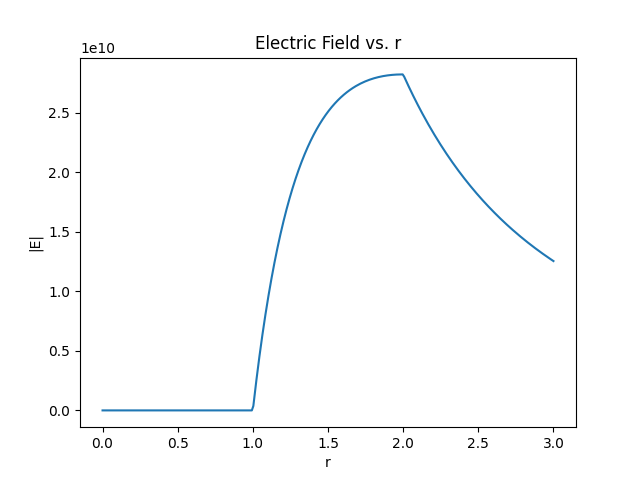
\includegraphics[width=0.45\textwidth]{./images/s2_15.png}
		\end{center}
		\caption{Electric Field \( | \mathbf{E} | \) vs \( r \)}\label{fig:s2_15}
	\end{figure}

\end{hwkProblem}
\begin{hwkProblem}{2.17}{}

	An infinite plane slab, of thickness \( 2d \), carries a uniform volume charge density \( \rho \). Find the electric field, as a function of \( y \), where \( y=0 \) at the center. Plot \( E \) versus \( y \), calling \( E \) positive when it points in the \( +y \) direction and negative when it points in the \( -y \) direction.

	\hwkSol

		\[
	\text{For } |y|\le d:\quad E(y)=\frac{\rho\,y}{\epsilon_0}.
	\]
	\[
	\text{For } |y|\ge d:\quad E(y)=\frac{\rho\,d}{\epsilon_0}\,\mathrm{sgn}(y).
	\]
	\hwkPart
	
	\begin{figure}[ht]
		\begin{center}
			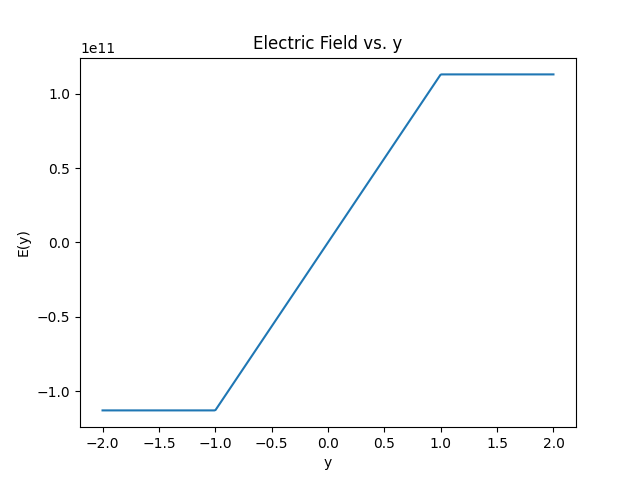
\includegraphics[width=0.45\textwidth]{./images/s2_17.png}
		\end{center}
		\caption{Electric Field \( E(y) \) vs \( y \)}\label{fig:s2_17}
	\end{figure}

\end{hwkProblem}
\begin{hwkProblem}{2.21}{}

	Find the potential inside and outside a uniformly charged solid sphere whose radius is \( R \) and whose total charge is \( q \). Use infinity as your reference point. Compute the gradient of \( V \) in each region, and check that it yields the correct field. Sketch \( V(r) \).

	\hwkSol

	\hwkPart
	\[
	\text{For } r\ge R:\quad V(r)=\frac{q}{4\pi\epsilon_0}\frac{1}{r}.
	\]
	\[
	\text{For } r\le R:\quad V(r)=\frac{q}{4\pi\epsilon_0}\frac{3R^2-r^2}{2R^3}.
	\]
	\hwkPart

	\[
	-\frac{dV}{dr}\Bigl|_{r\ge R}=\frac{q}{4\pi\epsilon_0}\frac{1}{r^2}=E(r),\qquad
	-\frac{dV}{dr}\Bigl|_{r\le R}=\frac{q}{4\pi\epsilon_0}\frac{r}{R^3}=E(r).
	\]

	\hwkPart
	
	\begin{figure}[ht]
		\begin{center}
			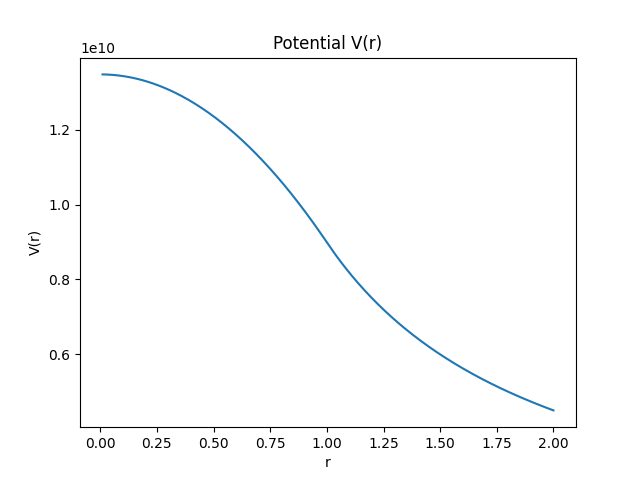
\includegraphics[width=0.45\textwidth]{./images/s2_21.png}
		\end{center}
		\caption{Potential \( V(r) \)}\label{fig:s2_21}
	\end{figure}

\end{hwkProblem}
\end{document}
